\documentclass[conference]{IEEEtran}

\usepackage{cite}
\usepackage{amsmath,amssymb,amsfonts}
\usepackage{algorithmic}
\usepackage{graphicx}
\usepackage{textcomp}
\usepackage{xcolor}
\usepackage{booktabs}
\usepackage{siunitx}
\usepackage{float}
\usepackage[hidelinks]{hyperref}

%================  CUSTOMIZATION  =================================================%

\def\BibTeX{{\rm B\kern-.05em{\sc i\kern-.025em b}\kern-.08em
    T\kern-.1667em\lower.7ex\hbox{E}\kern-.125emX}}

\sisetup{
  detect-all,       % matches the surrounding font
  separate-uncertainty = true,
  per-mode = symbol  % m/s instead of m s^-1
}

\graphicspath{{Figures/}{../Common_assets/}}

% Generic upright subscript macros
\newcommand{\Ax}[1]{A_\mathrm{#1}}
\newcommand{\Ix}[1]{I_\mathrm{#1}}
\newcommand{\Px}[1]{P_\mathrm{#1}}
\newcommand{\Rx}[1]{R_\mathrm{#1}}
\newcommand{\rx}[1]{r_\mathrm{#1}}
\newcommand{\Vx}[1]{V_\mathrm{#1}}
\newcommand{\Zx}[1]{Z_\mathrm{#1}}
\newcommand{\gx}[1]{g_\mathrm{#1}}

%================  START OF DOCUMENT  =============================================%
\begin{document}

\title{Elektroniske enheter og kretser\\
Lab 04: Characterisation of JFETs and Analysis of a Two-Stage Amplifier}

\author{\IEEEauthorblockN{Sølve Kjelseth}
\IEEEauthorblockA{\textit{Faculty of Technology, Natural Sciences and Maritime Sciences} \\
\textit{University of South-Eastern Norway}\\
Horten, Norway\\
274153@usn.no}
}

\maketitle

%================  ABSTRACT  ======================================================%

\begin{abstract}
This report presents the experimental characterisation of junction field-effect transistors (JFETs) and the analysis of a two-stage amplifier constructed from these devices.  
Individual transistor parameters were first determined by measuring the maximum drain current, and by estimating the threshold gate-source voltage, under different circuit configurations.  
The measured results provided the basis for modelling and bias point calculations.  

A two-stage amplifier was then designed and built using the characterised transistors.  
The DC bias of each stage was calculated by solving the system of transistor equations, and the results were compared with direct measurements of node voltages and drain currents.  
Most deviations were small and attributed to measurement uncertainty, with one larger difference observed but still within the expected limits of the theoretical model.  

Finally, the small-signal voltage gain of the amplifier was analysed and verified experimentally.  
Stage-by-stage calculations and total gain measurements showed close agreement, with differences within ten percent.  
The results demonstrate both the applicability of the JFET quadratic model for bias analysis and the practical challenges in measuring and interpreting transistor behaviour in laboratory conditions.  
\end{abstract}

%================  KEYWORDS  ======================================================%
\begin{IEEEkeywords}
JFET, transistor parameters, device modelling, bias analysis, small-signal gain
\end{IEEEkeywords}

%================  INTRODUCTION  ==================================================%
\section{Introduction}
% #region

Field-effect transistors are widely used in electronic circuits due to their high input impedance and favourable small-signal characteristics.  
Understanding their behaviour under different operating conditions is important for both circuit design and device modelling.  
In particular, the junction field-effect transistor (JFET) is well suited for laboratory analysis because of its relatively simple structure and well-defined current-voltage relationship.  

Accurate characterisation of JFET parameters provides the foundation for predicting circuit behaviour.  
Key quantities such as the maximum drain current and the threshold gate-source voltage are central to establishing operating points and designing amplifiers.  
Experimental determination of these parameters also offers valuable insight into how theoretical models compare with practical devices.  

Amplifiers form one of the most common applications of transistors, and their performance depends strongly on correct biasing and device parameters.  
A two-stage amplifier configuration allows for analysis of both individual transistor stages and overall circuit gain, providing a broader perspective on design and verification.  

This report documents the characterisation of JFET devices and their application in a two-stage amplifier.  
The work includes measurement of transistor parameters, determination of DC bias points using both calculations and direct measurements, and an evaluation of small-signal voltage gain.  
The results are used to compare theoretical predictions with practical outcomes and to highlight key considerations in experimental circuit analysis.   


%================  SUBSECTION  ====================================================%
\subsection{Determining individual FET characteristics}
% #region

The resistor values and the supply voltage were measured prior to the experiment, and the results are listed in Table~\ref{tab:global}.  

A JFET test circuit was first constructed using transistor \(Q_1\) to determine its maximum drain current, \(\Ix{DSS}\).  
In this configuration, the gate and source terminals were connected to ground, while a resistor \(\Rx{D}\) was inserted between the drain and the supply voltage \(\Vx{DD}\).  
The drain voltage \(\Vx{D}\) was measured, and the drain current \(\Ix{D}\) was calculated using (\ref{eq:id_calc}).  
Since \(\Vx{GS} = \qty{0}{\volt}\), the measured \(\Ix{D}\) equals \(\Ix{DSS}\).  
The corresponding results are presented in Table~\ref{tab:transistor1} under the section “Without \(\Rx{S}\)”.  

The circuit was then modified by including a source resistor \(\Rx{S}\) to enable estimation of the threshold gate-source voltage \(\Vx{GS(off)}\).  
In this case, both the gate-source voltage \(\Vx{GS}\) and the drain voltage \(\Vx{D}\) were measured, while the drain current \(\Ix{D}\) was again calculated using (\ref{eq:id_calc}).  
The value of \(\Vx{GS(off)}\) was then estimated from (\ref{eq:vgsoff_calc}).  
The resulting measurements and calculations are included in Table~\ref{tab:transistor1} under the section “With \(\Rx{S}\)”.  

The same procedure was repeated for a second transistor of the same type, designated \(Q_2\).  
Its measured and calculated values are summarised in Table~\ref{tab:transistor2}.  


\begin{equation}
    \label{eq:id_calc}
    \Ix{D} = \frac{\Vx{DD} - \Vx{D}}{\Rx{D}}
\end{equation}

\begin{equation}
    \label{eq:vgsoff_calc}
    \Vx{GS(off)} = \frac{\Vx{GS}}{1 - \sqrt{\tfrac{\Ix{D}}{\Ix{DSS}}}}
\end{equation}

\begin{figure}[!t]
    \centering
    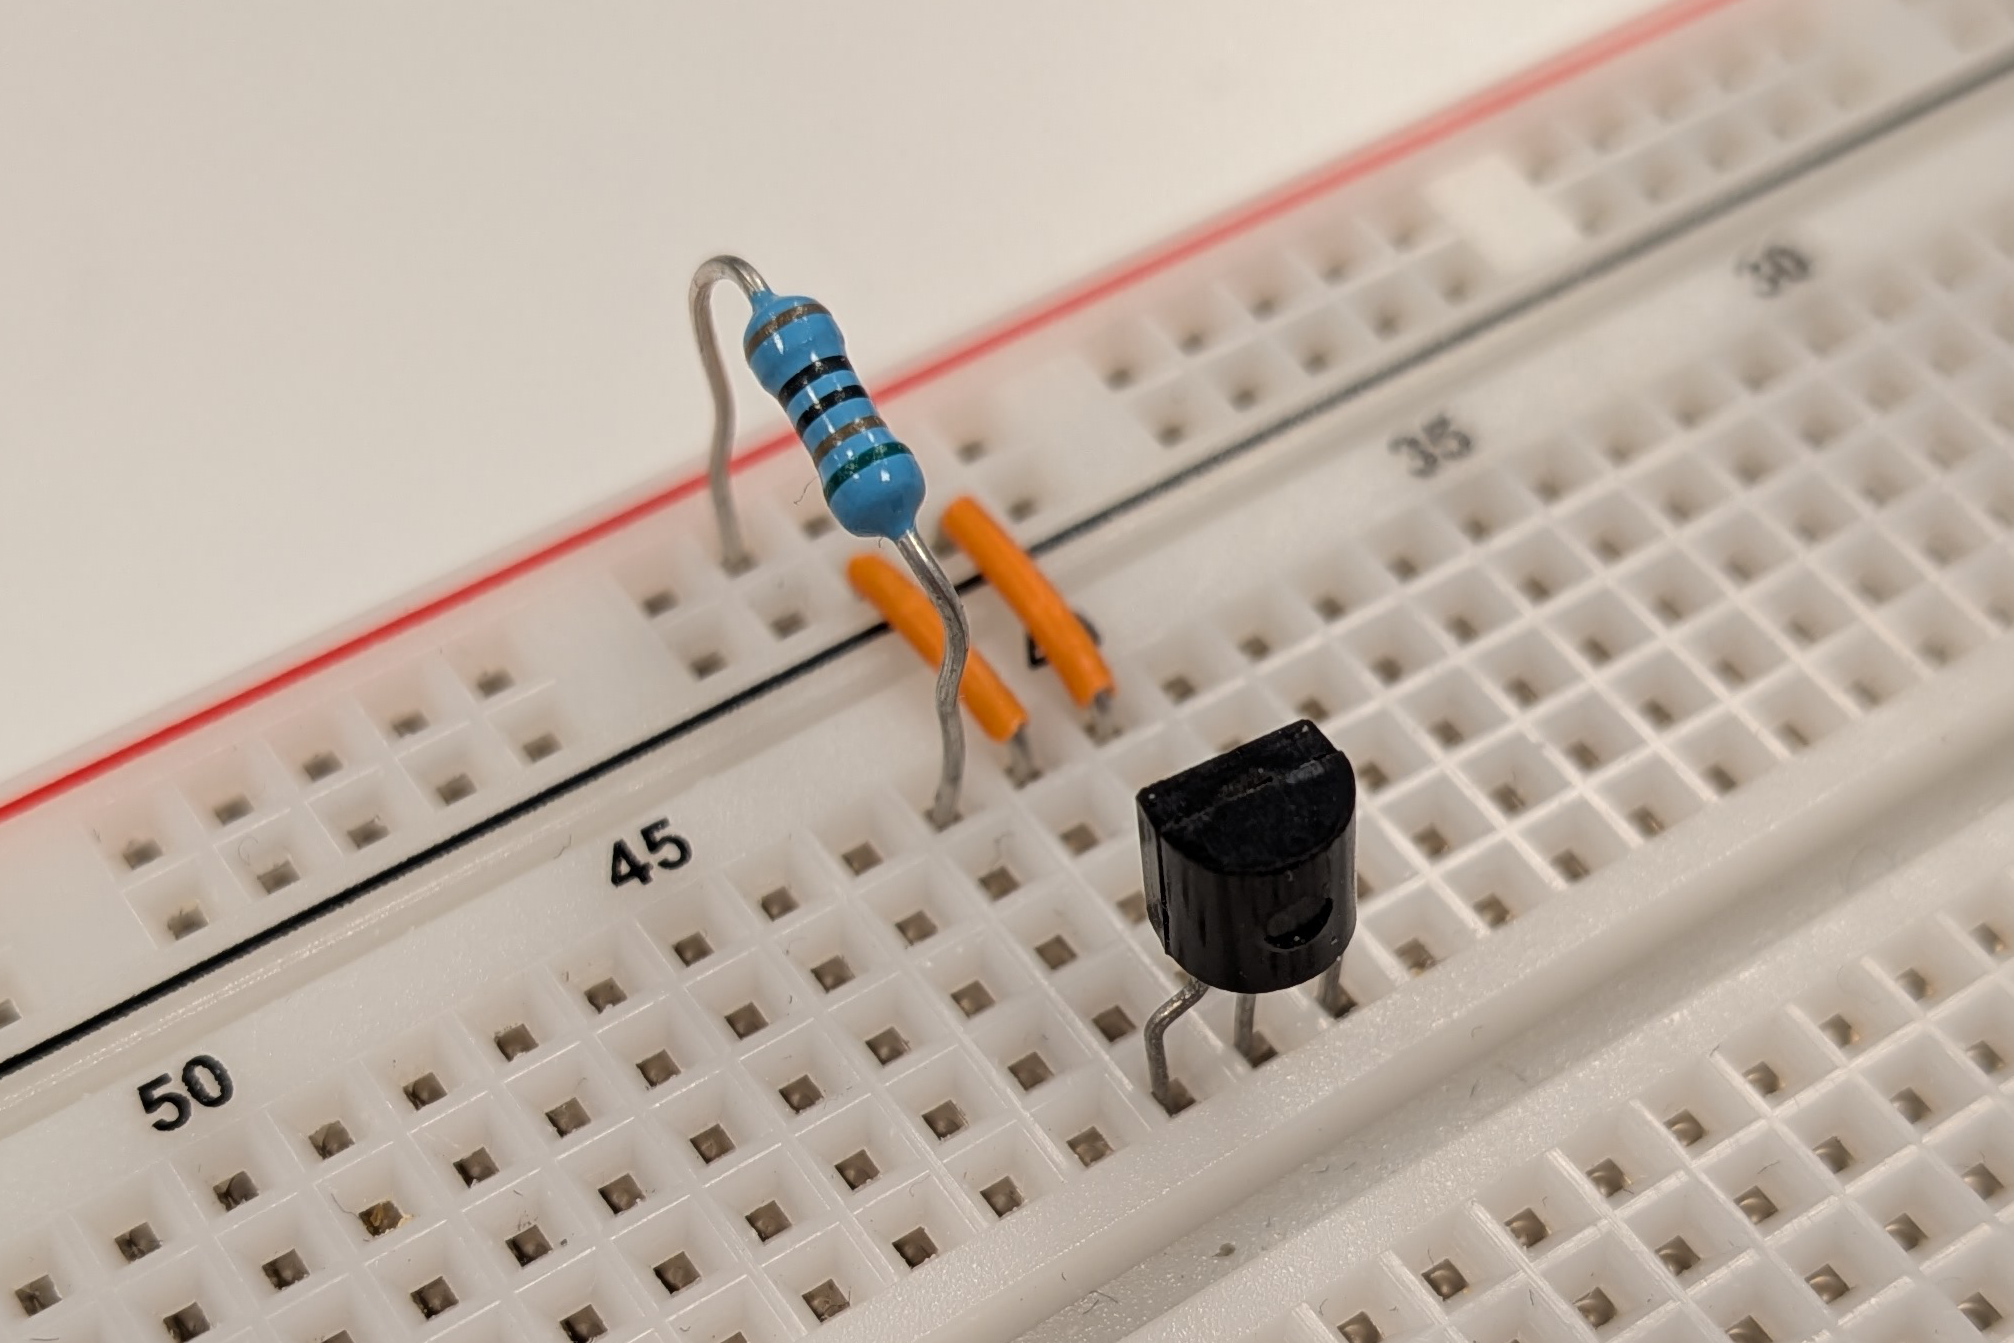
\includegraphics[width=0.9\linewidth]{Circuit1nores.jpg}
    \caption{Photograph of the experimental setup without source resistor, used to determine the maximum drain current.}
    \label{fig:circuit_idss}
\end{figure} 

\begin{table}[!t]
    \centering
    \caption{Global measured values}
    \label{tab:global}
    \begin{tabular}{l S[table-format=4.3] l}
        \toprule
        Parameter & {Value} & Unit \\
        \midrule
        \(\Rx{D}\) & 508.52 & \(\unit{\ohm}\) \\
        \(\Rx{S}\) & 981.9  & \(\unit{\ohm}\) \\
        \(\Vx{DD}\) & 10.03 & \(\unit{\volt}\) \\
        \bottomrule
    \end{tabular}
\end{table}

\begin{table}[!t]
    \centering
    \caption{Measured and calculated values for transistor~1}
    \label{tab:transistor1}
    \begin{tabular}{l S[table-format=3.3] l}
        \toprule
        Parameter & {Value} & Unit \\
        \midrule
        \multicolumn{3}{l}{\textit{Without \(\Rx{S}\): maximum current throughput}} \\
        \(\Vx{D}\)   & 6.48  & \(\unit{\volt}\) \\
        \(\Ix{D}\)   & 6.981 & \(\unit{\milli\ampere}\) \\
        \(\Ix{DSS}\) & 6.981 & \(\unit{\milli\ampere}\) \\
        \midrule
        \multicolumn{3}{l}{\textit{With \(\Rx{S}\): threshold gate-source voltage}} \\
        \(\Vx{GS}\)      & -1.587 & \(\unit{\volt}\) \\
        \(\Vx{D}\)       & 9.21   & \(\unit{\volt}\) \\
        \(\Ix{D}\)       & 1.613  & \(\unit{\milli\ampere}\) \\
        \(\Vx{GS(off)}\) & -3.056 & \(\unit{\volt}\) \\
        \bottomrule
    \end{tabular}
\end{table}

\begin{table}[!t]
    \centering
    \caption{Measured and calculated values for transistor~2}
    \label{tab:transistor2}
    \begin{tabular}{l S[table-format=3.3] l}
        \toprule
        Parameter & {Value} & Unit \\
        \midrule
        \multicolumn{3}{l}{\textit{Without \(\Rx{S}\): maximum current throughput}} \\
        \(\Vx{D}\)   & 6.09  & \(\unit{\volt}\) \\
        \(\Ix{D}\)   & 7.748 & \(\unit{\milli\ampere}\) \\
        \(\Ix{DSS}\) & 7.748 & \(\unit{\milli\ampere}\) \\
        \midrule
        \multicolumn{3}{l}{\textit{With \(\Rx{S}\): threshold gate-source voltage}} \\
        \(\Vx{GS}\)      & -1.640 & \(\unit{\volt}\) \\
        \(\Vx{D}\)       & 9.19   & \(\unit{\volt}\) \\
        \(\Ix{D}\)       & 1.652  & \(\unit{\milli\ampere}\) \\
        \(\Vx{GS(off)}\) & -3.047 & \(\unit{\volt}\) \\
        \bottomrule
    \end{tabular}
\end{table}

\begin{figure}[!t]
    \centering
    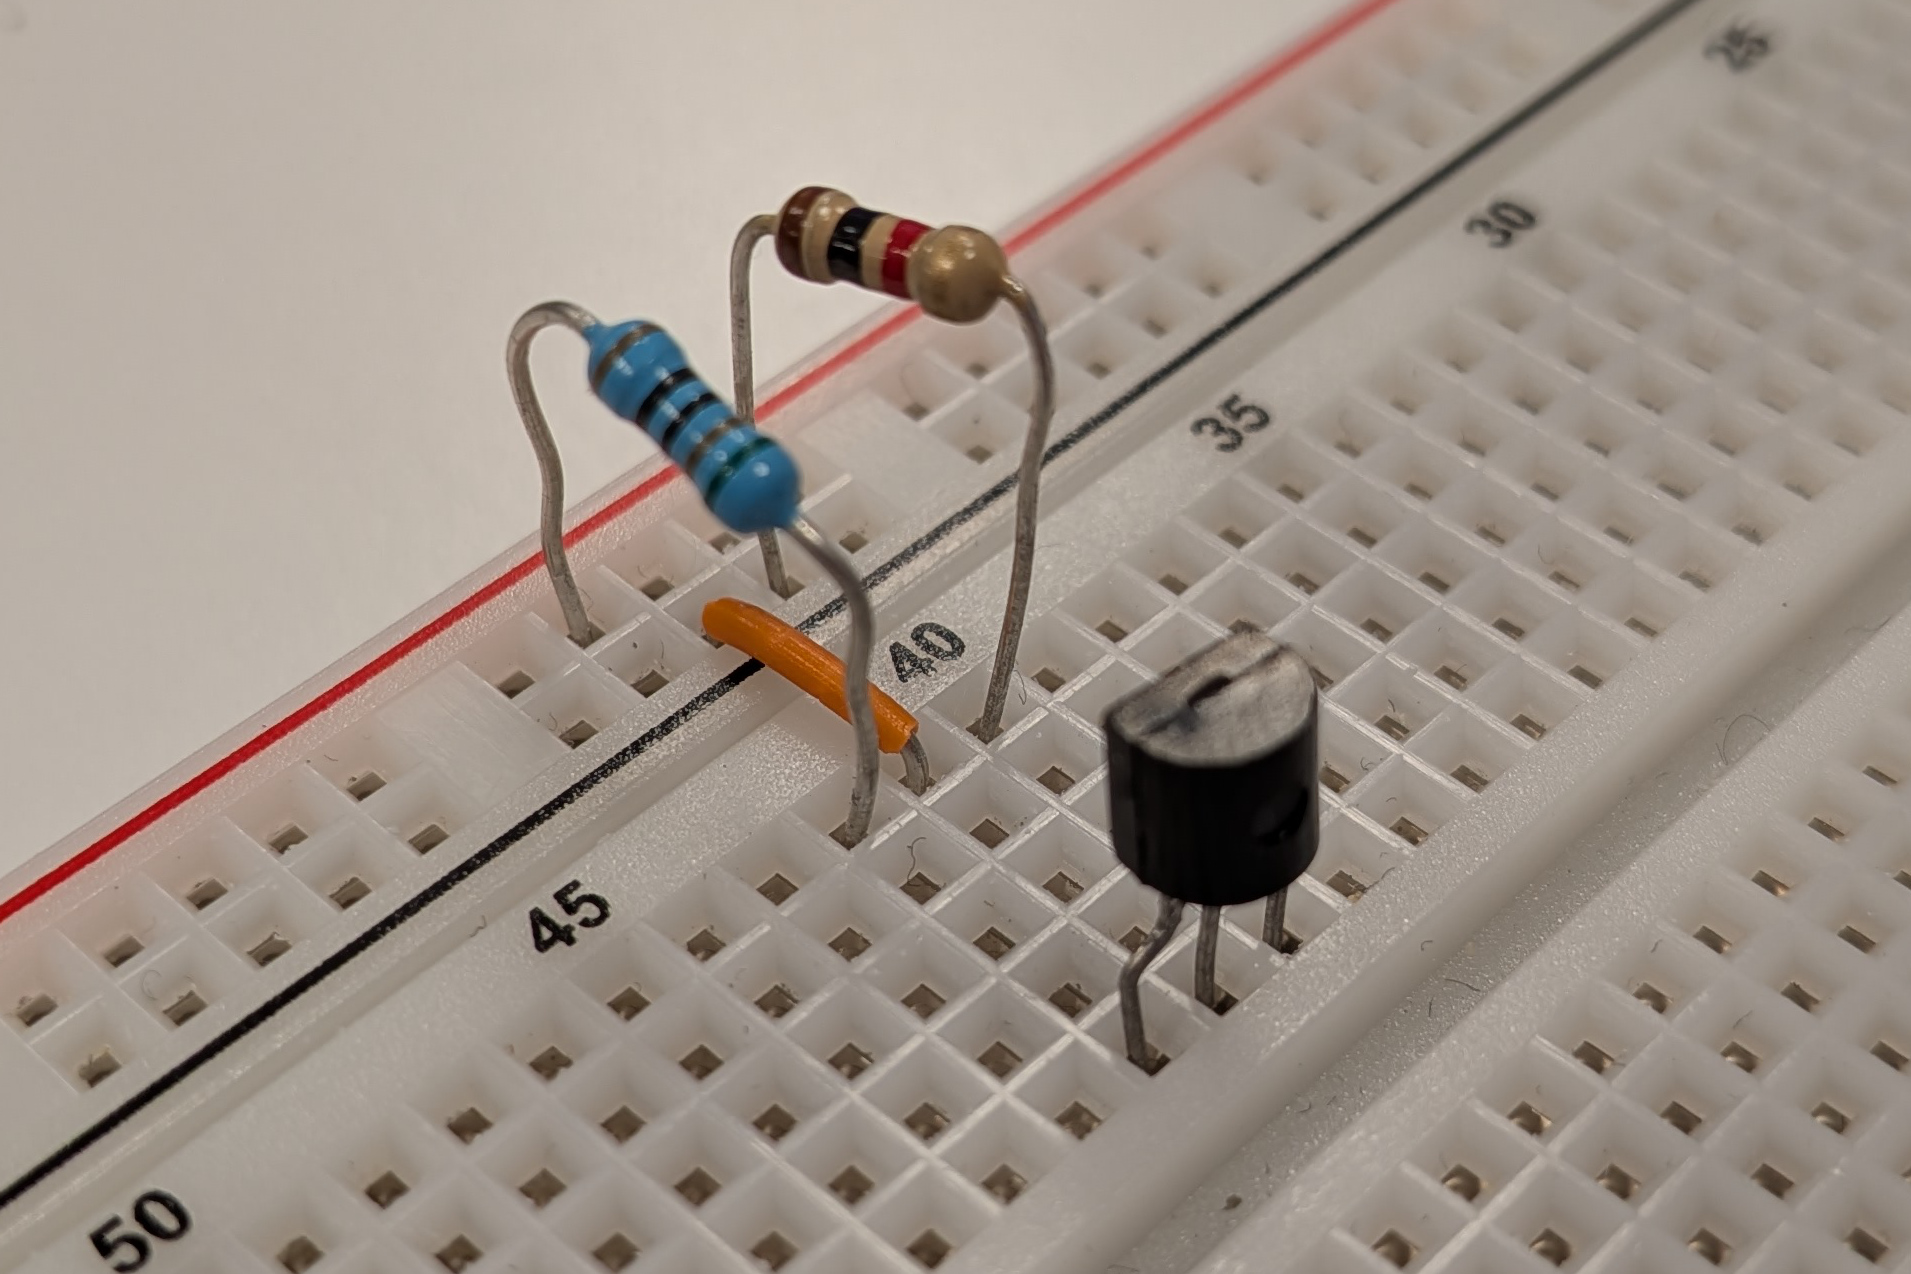
\includegraphics[width=0.9\linewidth]{Circuit1withres.jpg}
    \caption{Photograph of the experimental setup with source resistor, used to determine the cut-off gate-source voltage.}
    \label{fig:circuit_vgsoff}
\end{figure}

% #endregion

%================  SUBSECTION  ====================================================%
\subsection{DC bias of a two-stage amplifier circuit}
% #region

A two-stage amplifier circuit was constructed using the previously characterised transistors.  
All resistors and the supply voltage were measured beforehand, and the values are listed in Table~\ref{tab:global2}.  

The DC bias points were obtained by solving the system of equations given by the JFET characteristic in (\ref{eq:id_quad}) together with the node-voltage relation in (\ref{eq:vgs_eq}).  
The calculations were carried out with a computer algebra system (CAS) in GeoGebra, and a screenshot of the solution process is shown in Figure~\ref{fig:geogebra}.  
This system reduces to a quadratic expression with two solutions; one lies outside the valid range (below \(\Vx{GS(off)}\)) and was therefore discarded.  
The remaining valid solutions for \(\Vx{GS}\) and \(\Ix{D}\) were then used to determine the drain voltages \(\Vx{D}\).  

After the calculations, the amplifier circuit was built and node voltages were measured for both transistors.  
For each device, the values of \(\Vx{G}\), \(\Vx{S}\), \(\Vx{D}\), and \(\Vx{GS}\) were recorded directly, while the drain current was calculated using (\ref{eq:id_vsrs}).  
The corresponding results are presented in Table~\ref{tab:Q1Q2meas}.  

During measurements, the gate voltage of transistor \(Q_2\) proved difficult to obtain accurately with the coupling capacitor connected between the two stages.  
To achieve a stable reading of \(\Vx{G}\), the capacitor had to be temporarily removed.  

To compare the measured and calculated bias points, the relative difference was computed using (\ref{eq:diff}), where \(M\) denotes the measured value and \(C\) the calculated (theoretical) value.  
The differences are summarised in Table~\ref{tab:Q1Q2diff}.  
Most deviations are small and can be attributed to measurement uncertainties.  
The larger discrepancy observed in \(\Ix{D}\) for \(Q_2\) remains unexplained, but is still within reasonable limits for a theoretical model.

\begin{equation}
    \label{eq:id_quad}
    \Ix{D} = \Ix{DSS}\left( 1 - \frac{\Vx{GS}}{\Vx{GS(off)}} \right)^{2}
\end{equation}

\begin{equation}
    \label{eq:vgs_eq}
    \Vx{GS} = - \Ix{D} \cdot \Rx{S}
\end{equation}

\begin{equation}
    \label{eq:id_vsrs}
    \Ix{D} = \frac{\Vx{S}}{\Rx{S}}
\end{equation}

\begin{equation}
    \label{eq:diff}
    \text{Difference (}\unit{\percent}\text{)} =
    \frac{M - C}{C} \cdot 100
\end{equation} 

\begin{figure}[!t]
    \centering
    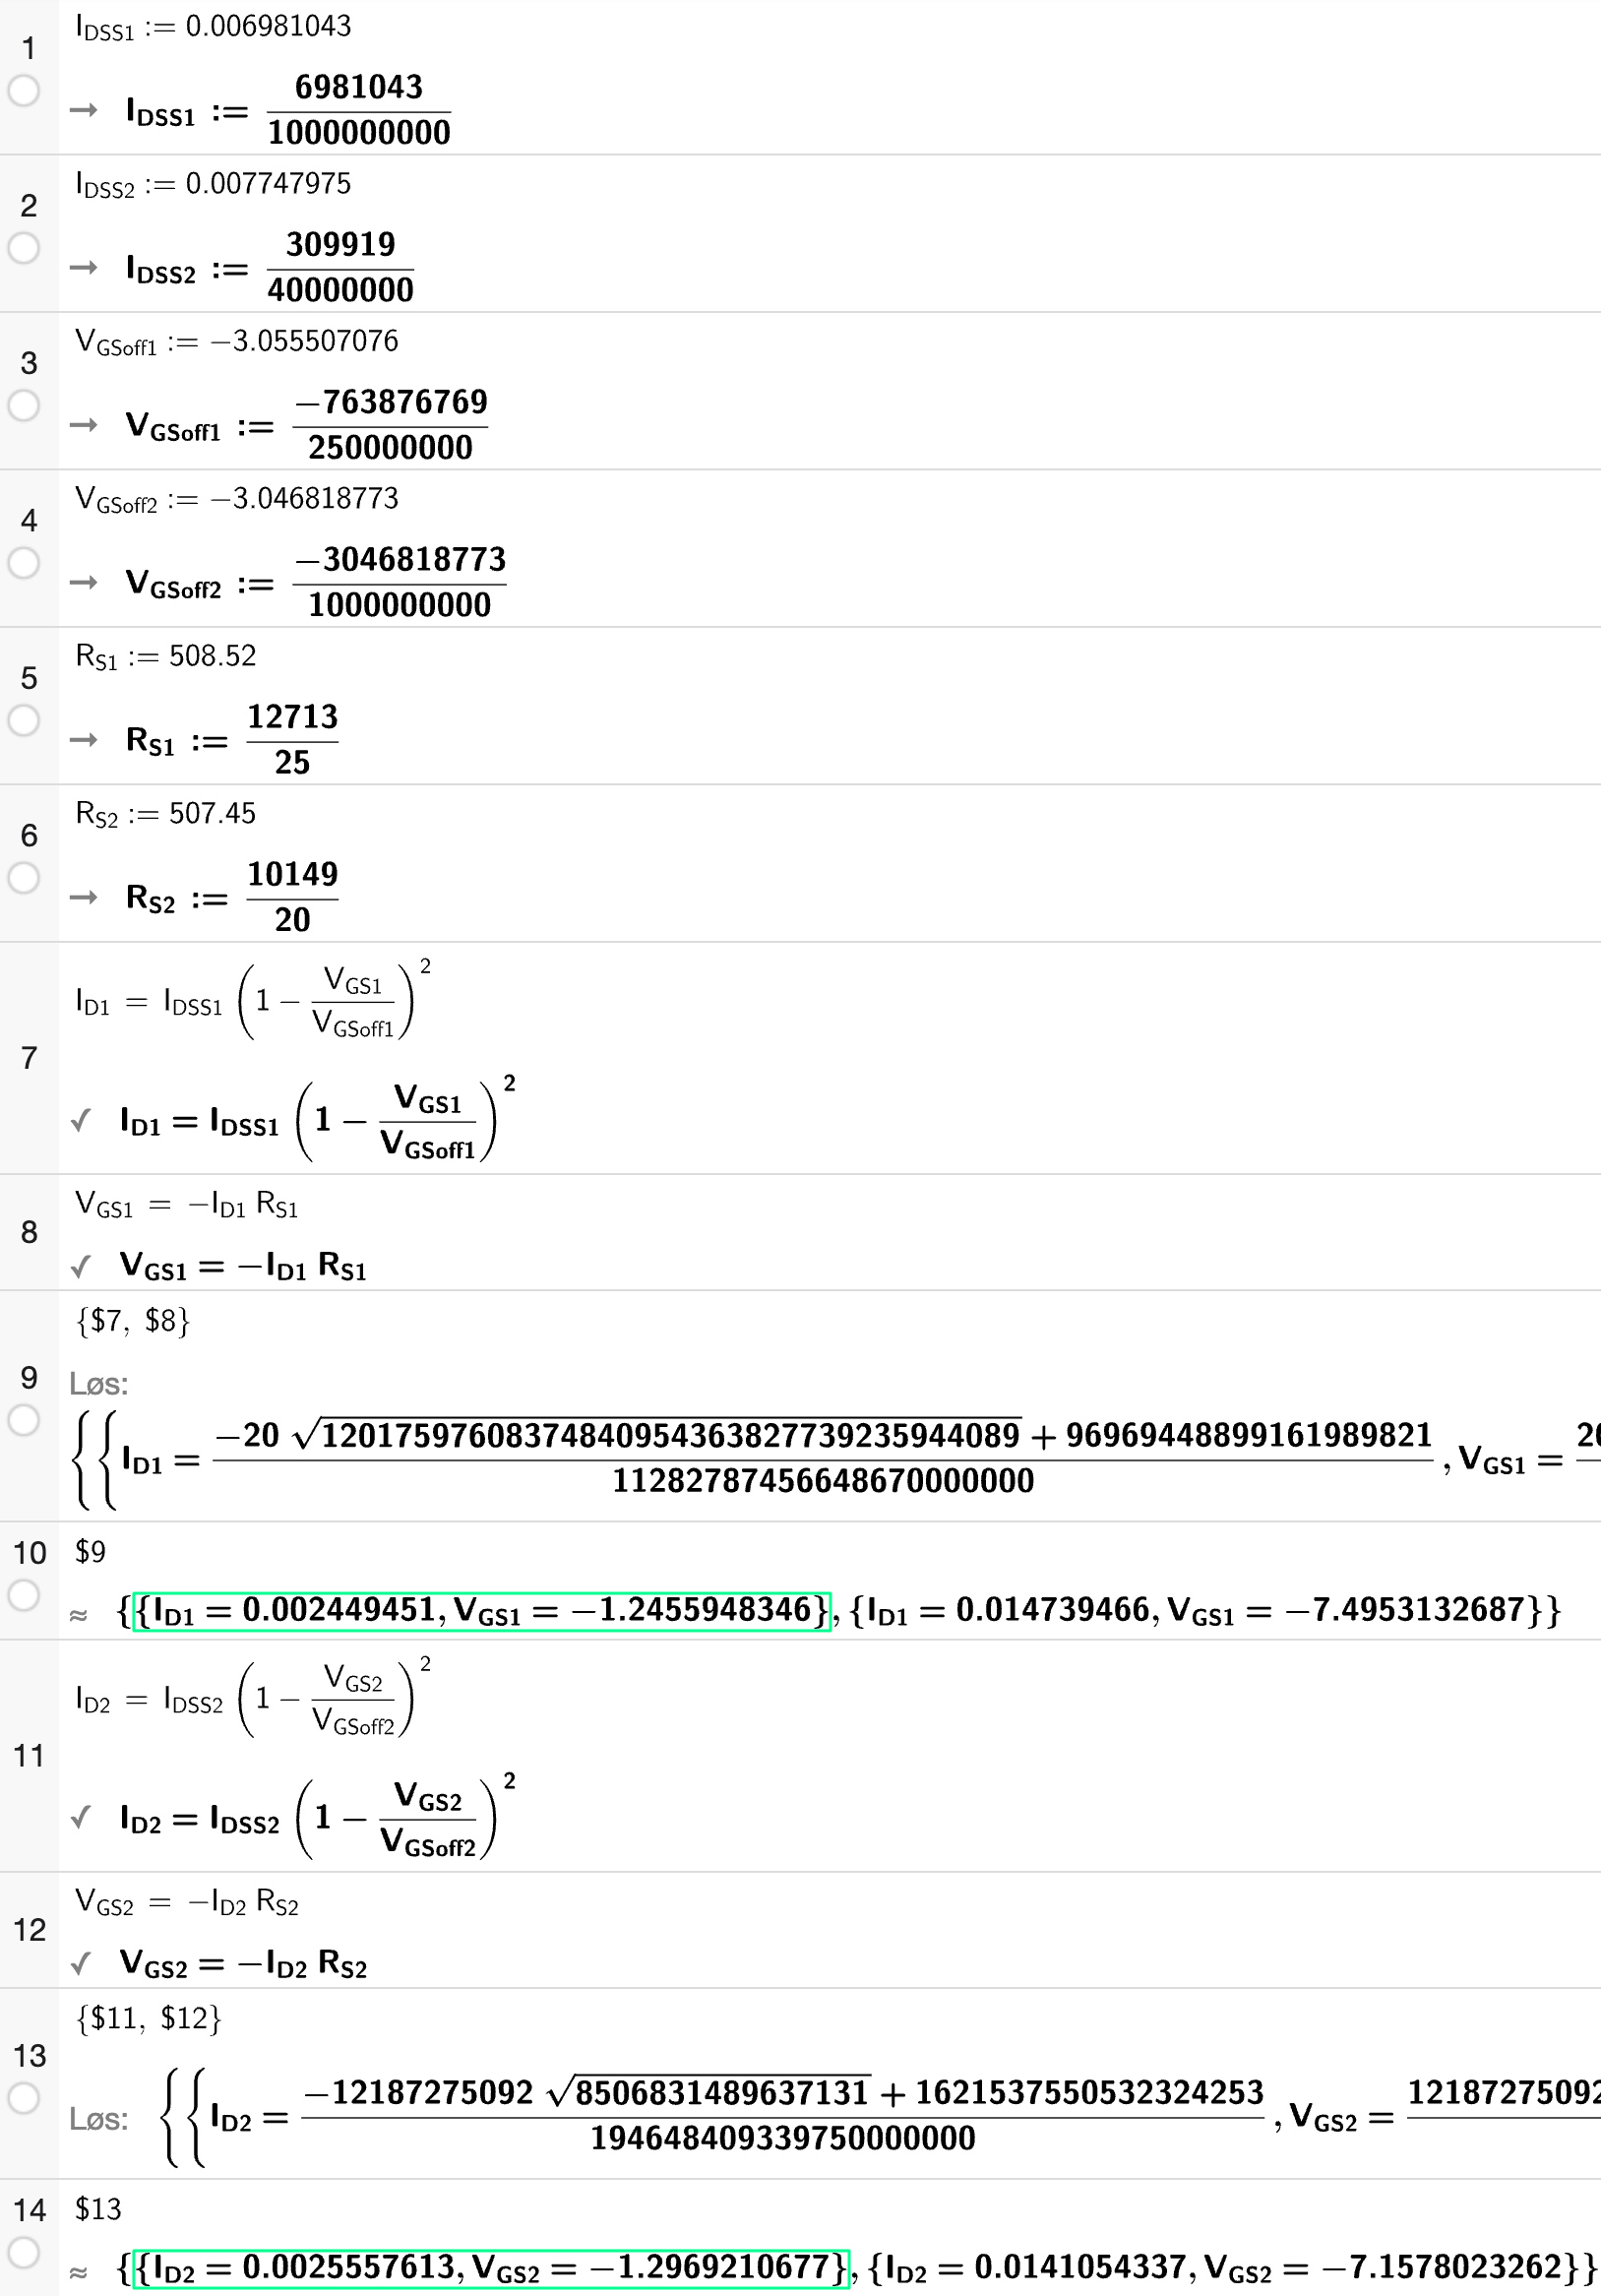
\includegraphics[width=0.9\linewidth]{GeoGebra.jpg}
    \caption{Screenshot from GeoGebra showing the solution process for the bias equations.}
    \label{fig:geogebra}
\end{figure}

\begin{figure}[!t]
    \centering
    
\includegraphics[width=0.9\linewidth]{Circuit2.jpg}
    \caption{Photograph of the constructed two-stage amplifier used for DC bias analysis.}
    \label{fig:amp_circuit}
\end{figure}

%================  TABLES  ========================================================%

\begin{table}[!t]
    \centering
    \caption{Global measured values for the two-stage amplifier}
    \label{tab:global2}
    \begin{tabular}{l S[table-format=4.2] l}
        \toprule
        Parameter & {Value} & Unit \\
        \midrule
        \(\Vx{DD}\)  & 19.98   & \(\unit{\volt}\) \\
        \(\Rx{G1}\)  & 1021.5  & \(\unit{\kilo\ohm}\) \\
        \(\Rx{G2}\)  & 1016.4  & \(\unit{\kilo\ohm}\) \\
        \(\Rx{S1}\)  & 508.52  & \(\unit{\ohm}\) \\
        \(\Rx{S2}\)  & 507.45  & \(\unit{\ohm}\) \\
        \(\Rx{D1}\)  & 2224.3  & \(\unit{\ohm}\) \\
        \(\Rx{D2}\)  & 2213.4  & \(\unit{\ohm}\) \\
        \(\Rx{L}\)   & 9889.1  & \(\unit{\ohm}\) \\
        \bottomrule
    \end{tabular}
\end{table}

\begin{table}[!t]
    \centering
    \caption{Calculated bias values for transistors}
    \label{tab:Q1Q2calc}
    \begin{tabular}{l S[table-format=3.4] l}
        \toprule
        Parameter & {Value} & Unit \\
        \midrule
        \multicolumn{3}{l}{\textit{Transistor \(Q_1\):}} \\
        \(\Ix{D}\)  & 2.449   & \(\unit{\milli\ampere}\) \\
        \(\Vx{GS}\) & -1.246  & \(\unit{\volt}\) \\
        \(\Vx{D}\)  & 14.532  & \(\unit{\volt}\) \\
        \midrule
        \multicolumn{3}{l}{\textit{Transistor \(Q_2\):}} \\
        \(\Ix{D}\)  & 2.556   & \(\unit{\milli\ampere}\) \\
        \(\Vx{GS}\) & -1.297  & \(\unit{\volt}\) \\
        \(\Vx{D}\)  & 14.323  & \(\unit{\volt}\) \\
        \bottomrule
    \end{tabular}
\end{table}

\begin{table}[!t]
    \centering
    \caption{Measured bias values for transistors}
    \label{tab:Q1Q2meas}
    \begin{tabular}{l S[table-format=3.4] l}
        \toprule
        Parameter & {Value} & Unit \\
        \midrule
        \multicolumn{3}{l}{\textit{Transistor \(Q_1\):}} \\
        \(\Vx{G}\)  & 0.500  & \(\unit{\milli\volt}\) \\
        \(\Vx{S}\)  & 1.275  & \(\unit{\volt}\) \\
        \(\Vx{D}\)  & 14.40  & \(\unit{\volt}\) \\
        \(\Vx{GS}\) & -1.228 & \(\unit{\volt}\) \\
        \(\Ix{D}\)  & 2.507  & \(\unit{\milli\ampere}\) \\
        \midrule
        \multicolumn{3}{l}{\textit{Transistor \(Q_2\):}} \\
        \(\Vx{G}\)  & 0.600  & \(\unit{\milli\volt}\) \\
        \(\Vx{S}\)  & 1.459  & \(\unit{\volt}\) \\
        \(\Vx{D}\)  & 13.62  & \(\unit{\volt}\) \\
        \(\Vx{GS}\) & -1.233 & \(\unit{\volt}\) \\
        \(\Ix{D}\)  & 2.875  & \(\unit{\milli\ampere}\) \\
        \bottomrule
    \end{tabular}
\end{table}

\begin{table}[!t]
    \centering
    \caption{Difference in calculated and measured bias values}
    \label{tab:Q1Q2diff}
    \begin{tabular}{l S[table-format=3.2] l}
        \toprule
        Parameter & {Value} & Unit \\
        \midrule
        \multicolumn{3}{l}{\textit{Transistor \(Q_1\):}} \\
        \(\Ix{D}\)  &  2.36  & \(\unit{\percent}\) \\
        \(\Vx{GS}\) & -1.41  & \(\unit{\percent}\) \\
        \(\Vx{D}\)  & -0.91  & \(\unit{\percent}\) \\
        \midrule
        \multicolumn{3}{l}{\textit{Transistor \(Q_2\):}} \\
        \(\Ix{D}\)  & 12.50   & \(\unit{\percent}\) \\
        \(\Vx{GS}\) & -4.93  & \(\unit{\percent}\) \\
        \(\Vx{D}\)  & -4.91  & \(\unit{\percent}\) \\
        \bottomrule
    \end{tabular}
\end{table}

% #endregion

%================  SUBSECTION  ====================================================%
\subsection{Voltage gain analysis}
% #region

The voltage gain of the amplifier was analysed separately for each stage and then combined to obtain the total gain.  
The calculations were based on the previously determined values of \(\Ix{DSS}\) and \(\Vx{GS(off)}\), together with the measured \(\Vx{GS}\) and resistor values of the circuit.  

The small-signal transconductance \(\gx{m}\) for each transistor was first determined using (\ref{eq:gm1calc}).  
The stage gains \(\Ax{V1}\) and \(\Ax{V2}\) were then calculated using (\ref{eq:AV1calc}) and (\ref{eq:AV2calc}), respectively.  
In the expression for \(\Ax{V1}\), the input resistance of the second stage \(\Rx{IN(Q2)}\) formally appears in parallel with \(\Rx{D1}\) and \(\Rx{G2}\).  
However, as this input resistance is extremely large, its contribution is negligible and was omitted from the calculation.  
Finally, the overall gain \(\Ax{V}\) was obtained from (\ref{eq:AVcalc}).  
The calculated results are summarised in Table~\ref{tab:AVcalc}.   

The amplifier was subsequently connected to a signal generator, and three voltages were measured: the input signal \(\Vx{sig}\), the intermediate voltage between stages \(\Vx{o1}\), and the output voltage across the load resistor \(\Vx{RL}\).  
These values were used to determine the gain from (\ref{eq:AV}).  
The gain was calculated in two ways: first, the overall gain was obtained directly by using \(\Vx{RL}\) as the output and \(\Vx{sig}\) as the input.  
Second, the stage gains were calculated individually by using \(\Vx{o1}\) as the output for the first stage and as the input for the second stage, before combining them with (\ref{eq:AVcalc}).  
Although mathematically redundant, this procedure confirmed the stage-by-stage results.  
The measured gains are listed in Table~\ref{tab:AVmeas}, with the total gain reported once.  

The relative differences between calculated and measured values were obtained using (\ref{eq:diff}) and are summarised in Table~\ref{tab:AVdiff}.  
The deviations are modest, with the total gain differing by less than 10\%, which is within a reasonable margin considering measurement uncertainty and modelling assumptions.

\begin{equation}
\label{eq:gm1calc}
    \gx{m} = \left( \frac{2 \cdot \Ix{DSS}} {\left| \Vx{GS(off)} \right|}
    \left( 1 - \frac{\Vx{GS}} {\Vx{GS(off)}} \right) \right)
\end{equation}

\begin{equation}
\label{eq:AV1calc}
    \Ax{V1} = \gx{m} \cdot
    \left( \Rx{D1} \parallel \Rx{G2} \parallel \Rx{IN(Q2)} \right)
\end{equation}

\begin{equation}
\label{eq:AV2calc}
    \Ax{V2} = \gx{m} \cdot
    \left( \Rx{D2} \parallel \Rx{L} \right)
\end{equation}

\begin{equation}
\label{eq:AVcalc}
    \Ax{V} = \Ax{V1} \cdot \Ax{V2}
\end{equation}

\begin{equation}
\label{eq:AV}
    \Ax{V} = \frac{\Vx{o}}{\Vx{i}}
\end{equation}

\vfill
\newpage

\begin{table}[!t]
    \centering
    \caption{Calculated gains}
    \label{tab:AVcalc}
    \begin{tabular}{l S[table-format=3.3] l}
        \toprule
        Parameter & {Value} & Unit \\
        \midrule
        \(\Ax{V1}\)  & 6.066  & --- \\
        \(\gx{m1}\)  & 2.733  & \(\unit{\milli\siemens}\) \\
        \(\Ax{V2}\)  & 5.476  & --- \\
        \(\gx{m2}\)  & 3.028  & \(\unit{\milli\siemens}\) \\
        \(\Ax{V}\)   & 33.216 & --- \\
        \bottomrule
    \end{tabular}
\end{table}

\begin{table}[!t]
    \centering
    \caption{Measured gains}
    \label{tab:AVmeas}
    \begin{tabular}{l S[table-format=3.3] l}
        \toprule
        Parameter & {Value} & Unit \\
        \midrule
        \(\Ax{V1}\)  & 6.066  & --- \\
        \(\Ax{V2}\)  & 5.476  & --- \\
        \(\Ax{V}\)   & 33.216 & --- \\
        \bottomrule
    \end{tabular}
\end{table}

\begin{table}[!t]
    \centering
    \caption{Difference in measured and calculated gains}
    \label{tab:AVdiff}
    \begin{tabular}{l S[table-format=3.2] l}
        \toprule
        Parameter & {Value} & Unit \\
        \midrule
        \(\Ax{V1}\)  & 4.03 & \(\unit{\percent}\) \\
        \(\Ax{V2}\)  & 3.03 & \(\unit{\percent}\) \\
        \(\Ax{V}\)   & 7.18 & \(\unit{\percent}\) \\
        \bottomrule
    \end{tabular}
\end{table}

% #endregion


%================  SECTION  =======================================================%
\section{Conclusion}
% #region

This work has demonstrated the experimental characterisation of JFET devices and their use in a two-stage amplifier circuit.  
Key transistor parameters, including the maximum drain current and the threshold gate-source voltage, were measured and applied in theoretical bias calculations.  
The calculated bias points showed good agreement with direct measurements, with only minor deviations that can be attributed to measurement uncertainty and modelling limitations.  

The small-signal voltage gain of the amplifier was also analysed.  
Both stage-by-stage and overall gain results were in close agreement with theory, differing by less than ten percent.  
This confirms the validity of the quadratic model for JFET operation within the tested range, while also highlighting the importance of accurate parameter extraction.  

Overall, the results illustrate how device-level characterisation supports circuit-level analysis and provide a practical demonstration of the link between transistor models and amplifier performance.  
% #endregion



%================  ACKNOWLEDGMENT  ================================================%
\section*{Acknowledgment}
% #region
This report corresponds to Lab~04 in the course \emph{Elektroniske enheter og kretser}.
All related materials (\LaTeX~sources, raw data, figures, codes and more) are released under the MIT License and available at \url{https://github.com/Kjelseth/EEK_lab}.
% #endregion

\end{document}